\documentclass{article}
\usepackage{lmodern}
\usepackage[T1]{fontenc}
\usepackage{shapepar}
\usepackage{microtype}
\usepackage{lipsum}
\usepackage{pgfplots}
\pgfplotsset{compat=1.9}
\usepackage{tikz}
\usetikzlibrary{calc,fit,intersections,folding}
\usepackage{pstricks-add}
\usetikzlibrary{arrows.meta,angles,arrows,quotes,backgrounds}


\newcommand{\clrone}{blue}
\newcommand{\clrtwo}{red}

\begin{document}
\thispagestyle{empty}
    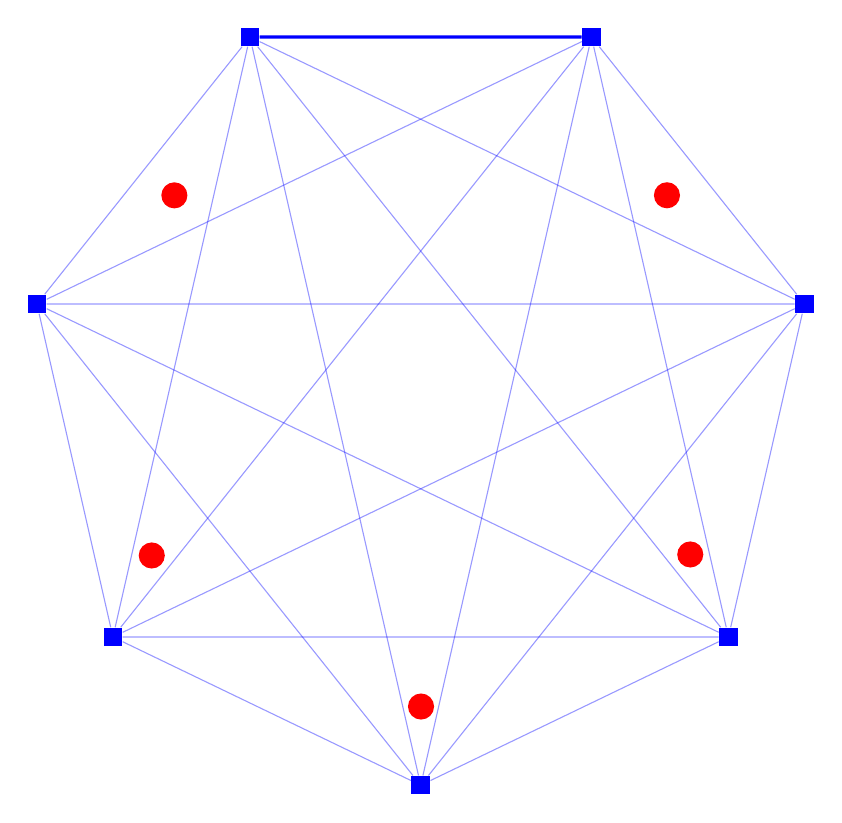
\begin{tikzpicture}[rotate = 12.86]
    %blue points
        \foreach \i in {1,...,7} {
            \node[fill, \clrone] (b\i) at (360*\i/7:5) {};
        }
    %edges between blue points
        %1 to 2..7
        \foreach \i in {2,...,7} {
            \draw[\clrone, opacity = 0.4] (b1) -- (b\i);
        }
        %2 to 3..7
        \foreach \i in {3,...,7} {
            \draw[\clrone, opacity = 0.4] (b2) -- (b\i);
        }
        %3 to 4..7
        \foreach \i in {4,...,7} {
            \draw[\clrone, opacity = 0.4] (b3) -- (b\i);
        }
        %4 to 5..7
        \foreach \i in {5,...,7} {
            \draw[\clrone, opacity = 0.4] (b4) -- (b\i);
        }
        %5 to 6..7
        \foreach \i in {6,...,7} {
            \draw[\clrone, opacity = 0.4] (b5) -- (b\i);
        }
        %6 to 7
        \foreach \i in {7} {
            \draw[\clrone, opacity = 0.4] (b6) -- (b\i);
        }
        \draw[very thick,\clrone] (b1) -- (b2);

        %red points placed by hand
        \node[circle, fill, \clrtwo] (r1) at (25.7:4) {};
        \node[circle, fill, \clrtwo] (r2) at (-44:4) {};
        \node[circle, fill, \clrtwo] (r3) at (-102.8:4) {};
        \node[circle, fill, \clrtwo] (r4) at (-161.5:4) {};
        \node[circle, fill, \clrtwo] (r5) at (128.6:4) {};
    \end{tikzpicture}
\end{document}